\documentclass[oneside,a4paper,14pt]{extarticle}
\usepackage[T1,T2A]{fontenc}
\usepackage[a4paper,letterpaper,top=20mm,bottom=20mm,left=30mm,right=10mm]{geometry}
\usepackage{amsmath, amssymb}
\usepackage[utf8]{inputenc}
\usepackage[russian]{babel}
\usepackage{textcomp}
\usepackage{indentfirst}
\usepackage{graphicx}
\usepackage{float}
\usepackage{mwe}
\usepackage{wrapfig}
\usepackage{caption}
\usepackage{tocloft}
\renewcommand{\cftsecleader}{\cftdotfill{\cftdotsep}}
\usepackage{longtable}
\usepackage{amsmath}
\usepackage{amsfonts}
\usepackage{amsthm}
\usepackage{float}
\usepackage[all]{xy}
\usepackage[breaklinks]{hyperref}
\usepackage{titlesec}
\usepackage{fancyvrb}
\usepackage{paracol}
\usepackage{listings}
\usepackage{xcolor}

\definecolor{codegreen}{rgb}{0,0.6,0}
\definecolor{codegray}{rgb}{0.5,0.5,0.5}
\definecolor{codepurple}{rgb}{0.58,0,0.82}
\definecolor{backcolour}{rgb}{0.95,0.95,0.92}

\lstdefinestyle{cppstyle}{
    backgroundcolor=\color{backcolour},
    commentstyle=\color{codegreen},
    keywordstyle=\color{magenta},
    numberstyle=\tiny\color{codegray},
    stringstyle=\color{codepurple},
    basicstyle=\ttfamily\footnotesize,
    breakatwhitespace=false,
    breaklines=true,
    captionpos=b,
    keepspaces=true,
    numbers=left,
    numbersep=5pt,
    showspaces=false,
    showstringspaces=false,
    showtabs=false,
    tabsize=2,
    language=C++
}

\lstset{style=cppstyle}

\titleformat{\section}{\normalsize\bfseries}{\thesection}{1em}{}
\titleformat{\subsection}{\normalsize\bfseries}{\thesubsection}{1em}{}
\titleformat{\subsubsection}{\normalsize\bfseries}{\thesubsubsection}{1em}{}
\renewcommand\baselinestretch{1.33}\normalsize
\setlength{\parindent}{1.25cm}

\begin{document}

\newpage\thispagestyle{empty}
\begin{center}
    МИНИСТЕРСТВО НАУКИ И ВЫСШЕГО ОБРАЗОВАНИЯ\\
    РОССИЙСКОЙ ФЕДЕРАЦИИ\\
    ФЕДЕРАЛЬНОЕ ГОСУДАРСТВЕННОЕ БЮДЖЕТНОЕ\\
    ОБРАЗОВАТЕЛЬНОЕ УЧРЕЖДЕНИЕ ВЫСШЕГО ОБРАЗОВАНИЯ\\
    «ВЯТСКИЙ ГОСУДАРСТВЕННЫЙ УНИВЕРСИТЕТ»\\
    Институт математики и информационных систем\\
    Факультет автоматики и вычислительной техники\\
    Кафедра электронных вычислительных машин
\end{center}

\vspace{20mm}
\begin{center}

    Отчёт по лабораторной работе №1\\
    по дисциплине\\
    «Объектно-ориентированное программирование»\\
\end{center}
\vfill

Выполнил студент гр. ИВТб-2301-05-00 \hfill
\makebox[8cm]{\hrulefill /Ковальский И.И./}

Проверил преподаватель\hfill
\makebox[8cm]{\hrulefill /Шмакова Н.А./}

\vfill
\begin{center}
    Киров\\
    2026
\end{center}

\newpage
\setcounter{page}{1}
\tableofcontents
\newpage

\section*{Цель работы}
\addcontentsline{toc}{section}{Цель работы}
Изучение принципов объектно-ориентированного программирования на языке C++.

\section*{Задание}
\addcontentsline{toc}{section}{Задание}

\begin{enumerate}
    \item Выбрать и согласовать с преподавателем предметную область.
    \item Создать иерархию классов, состоящую не менее чем из одного родительского и двух дочерних классов.
    \item В каждом классе определить не менее двух членов данных, не менее двух собственных, а для дочерних - не менее двух унаследованных и двух переопределенных (перекрытых) член-функций.
    \item Разработать приложение, демонстрирующее принципы инкапсуляции, наследования и полиморфизма.
\end{enumerate}

Примечания: работа с объектами осуществляется только через переменные родительского типа; каждый класс в отдельном файле; отчёт должен содержать описание предметной области, схему структуры иерархии классов, описание методов, особенности реализации.

\newpage

\section*{Выполнение лабораторной работы}
\addcontentsline{toc}{section}{Выполнение лабораторной работы}

\subsection*{Выбор предметной области}
\addcontentsline{toc}{subsection}{Выбор предметной области}
В качестве предметной области выбрана тема "Организации". В современном мире существует множество типов организаций, которые имеют общие черты, но различаются по целям, способам финансирования и распределения прибыли. Это позволяет наглядно продемонстрировать принципы наследования.

\subsection*{Создание иерархии классов}
\addcontentsline{toc}{subsection}{Создание иерархии классов}
Разработана иерархия, состоящая из одного абстрактного базового класса Organization и его дочерних классов: Commersorg (коммерческая организация) и Noncomersorg (некоммерческая организация).

\begin{figure}[H]
  \centering
  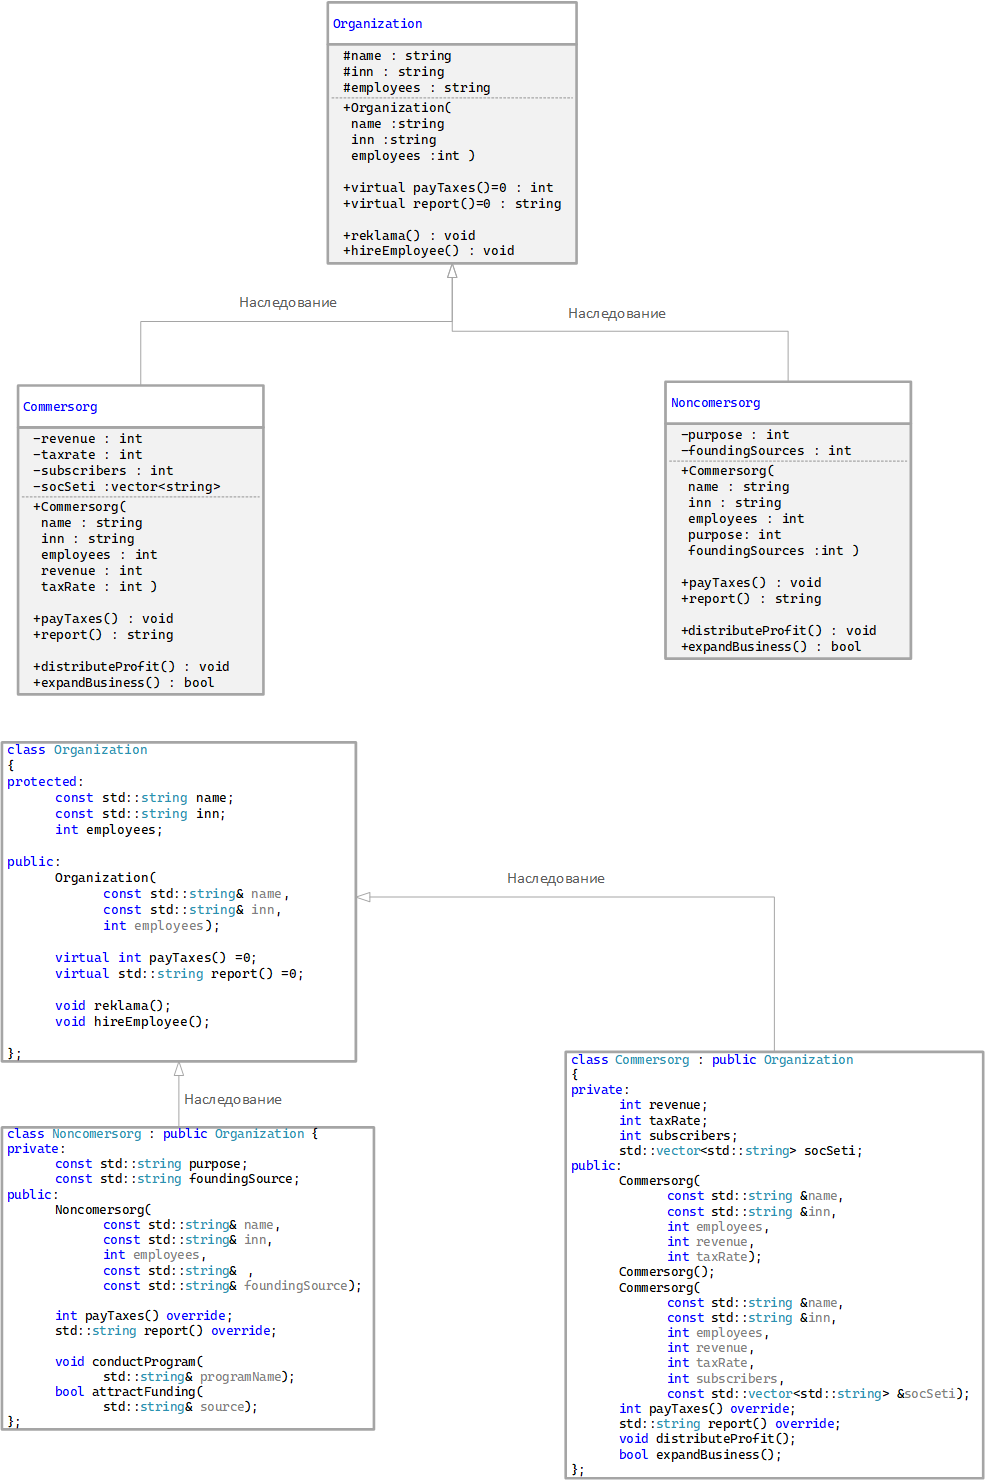
\includegraphics[width=0.8\textwidth]{Диаграмма классов.png}
  \caption{Диаграмма классов}
  \label{fig:diagram}
\end{figure}

\subsection*{Описание классов}
\addcontentsline{toc}{subsection}{Описание классов}

\subsubsection*{Базовый класс Organization: organization.h, organization.cpp}

\textbf{private поля:}
\begin{itemize}
    \item name (string) - название организации.
    \item inn (string) - ИНН организации.
    \item employees (int) - количество сотрудников.
\end{itemize}

\textbf{Конструкторы:}
\begin{itemize}
    \item Organization() - конструктор по умолчанию\\Инициализирует name = "Organization", inn = "1234567890", employees = 0.
    \item Organization(const string\& name, const string\& inn, int employees)\\Конструктор с параметрами. Устанавливает переданные значения полей класса.
    \item Organization(const Organization\& other)\\Конструктор копирования. Копирует поля из другого объекта.
\end{itemize}

\textbf{public деструктор:}
\begin{itemize}
    \item virtual ~Organization() \{\} - виртуальный деструктор.
\end{itemize}

\newpage

\textbf{public геттеры и сеттеры:}
\begin{itemize}
    \item getName() - возвращает string, название организации.
    \item getInn() - возвращает string, ИНН.
    \item getEmployees() - возвращает int, количество сотрудников.
    \item setName(const string\& newName) - void, устанавливает новое название.
    \item setInn(const string\& newInn) - void, устанавливает новый ИНН.
    \item setEmployees(int newEmployees) - void, устанавливает новое количество сотрудников.
\end{itemize}

\textbf{Виртуальные public методы :}
\begin{itemize}
    \item payTaxes() - возвращает int. Виртуальный метод, вычисляет сумму налога.
    \item report() - возвращает string. Формирует отчёт об организации.
\end{itemize}

\textbf{Общие public методы:}
\begin{itemize}
    \item hireEmployee() - void.\\Увеличивает employees на 1 и выводит сообщение о найме.
    \item reklama() - void.\\Выводит рекламную строку с названием организации.
\end{itemize}

\newpage

\subsubsection*{Класс Commersorg: commercial.h, commercial.cpp}

Наследование: public Organization.

\textbf{private поля:}
\begin{itemize}
    \item revenue (int) - выручка организации.
    \item taxRate (int) - налоговая ставка в процентах.
    \item subscribers (int) - количество подписчиков.
    \item socSeti (vector<string>) - список названий соцсетей.
\end{itemize}

Наследуемые поля от Organization: name, inn, employees. Они остаются private в базовом классе, доступ к ним через геттеры/сеттеры базового класса.

\textbf{Конструкторы:}
\begin{itemize}
    \item Commersorg() - конструктор по умолчанию.\\ Параметры создаваемого объекта: name="ООО Мурат Насыров", inn="458358238", employees=5, revenue=100, taxRate=1, subscribers=0, пустой вектор socSeti.
    \item Commersorg(const string\& name, const string\& inn, int employees, int revenue, int taxRate)\\Конструктор с параметрами, но без подписчиков и соцсетей.
    \item Commersorg(const string\& name, const string\& inn, int employees, int revenue, int taxRate, int subscribers, const vector<string>\& socSeti)\\Полный конструктор.
    \item Commersorg(const Commersorg\& other) - конструктор копирования.\\Копирует наследованную часть через конструктор копирования наследованного класса, затем копирует собственные поля.
\end{itemize}

\newpage

\textbf{Геттеры и сеттеры (public):}
\begin{itemize}
    \item getRevenue() - возвращает int, выручку.
    \item getTaxRate() - возвращает int, налоговую ставку.
    \item getSubscribers() - возвращает int, количество подписчиков.
    \item getSocSeti() - возвращает vector<string>, список соцсетей.
    \item setRevenue(int newRevenue) - void, устанавливает новую выручку.
    \item setTaxRate(int newTaxRate) - void, устанавливает новую налоговую ставку.
    \item setSubscribers(int newSubscribers) - void, устанавливает новое количество подписчиков.
    \item setSocSeti(const vector<string>\& newSocSeti) - void, заменяет список соцсетей.
    \item addSocSeti(const string\& social) - void, добавляет одну соцсеть в конец вектора.
\end{itemize}

\textbf{Переопределённые public виртуальные методы:}
\begin{itemize}
    \item payTaxes() - возвращает int. Реализация: revenue * taxRate / 100.
    \item report() - возвращает string. Формирует строку: "Коммерческая организация: " + getName() + ", Выручка: " + revenue + ", Сотрудники: " + getEmployees(). Если socSeti не пуст, добавляет ", Соцсети: " и перечисляет их через пробел.
\end{itemize}

\textbf{Собственные public методы:}
\begin{itemize}
    \item expandBusiness() - void.\\Увеличивает subscribers на 100 и выводит сообщение "Расширение выполнено! новые подписчики: " + значение subscribers.
    \item distributeProfit() - void.\\Выводит сообщение "Бюджет для распределения: " + значение revenue * 5.
\end{itemize}

\subsubsection*{Класс Noncomersorg: noncomersorg.h, noncomersorg.cpp}

Наследование: public Organization.

\textbf{private поля:}
\begin{itemize}
    \item purpose (string) - цель деятельности организации.
    \item foundingSource (string) - источник финансирования.
\end{itemize}

Наследуемые поля: name, inn, employees.

\textbf{Конструкторы:}
\begin{itemize}
    \item Noncomersorg() - конструктор по умолчанию.\\ Вызывает конструктор базового класса с параметрами: name="Фонд добра", inn="0987654321", employees=10,purpose="Цветы", foundingSource="Гранты".
    \item Noncomersorg(const string\& name, const string\& inn, int employees, const string\& purpose, const string\& foundingSource)\\ Конструктор с параметрами. Устанавливает собственные и наследованные поля.
    \item Noncomersorg(const Noncomersorg\& other) \\ Конструктор копирования. Копирует наследованную часть через конструктор копирования наследованного класса, копирует purpose и foundingSource.
\end{itemize}

\textbf{public геттеры и сеттеры:}
\begin{itemize}
    \item getPurpose() - возвращает string, цель организации.
    \item getFoundingSource() - возвращает string, источник финансирования.
    \item setPurpose(const string\& newPurpose) - void, устанавливает новую цель.
    \item setFoundingSource(const string\& newSource) - void, устанавливает новый источник финансирования.
\end{itemize}

\newpage

\textbf{Переопределённые public виртуальные методы:}
\begin{itemize}
    \item payTaxes() - возвращает int.\\Реализация: getEmployees() * 10.
    \item report() - возвращает string.\\Формирует строку: "Некоммерческая организация: " + getName() + ", цель: " + purpose + ", сотрудники: " + getEmployees() + ", Источники финансирования: " + foundingSource.
\end{itemize}

\textbf{Собственные public методы:}
\begin{itemize}
    \item conductProgram(const string\& programName) - void.\\Выводит сообщение "Программа: " + programName + "| | |Организация:" + getName().
    \item attractFunding(const string\& source) - void.\\Выводит сообщение "Привлечение финансирования из: " + source + "| | |Для: " + getName(), затем вызывает setFoundingSource(source) для обновления источника финансирования.
\end{itemize}

\newpage

\subsection*{Разработка демонстрационного приложения}
\addcontentsline{toc}{subsection}{Разработка демонстрационного приложения}

Для демонстрации созданной структуры разработано консольное приложение.

\textbf{Демонстрация инкапсуляции:}
Все данные классов (revenue, purpose и т.д.) объявлены в секции private. Доступ к ним и изменение возможны только через публичные методы-геттеры и сеттеры. Например, установить новую цель некоммерческой организации можно только через setPurpose, а прочитать - через getPurpose.

\textbf{Демонстрация наследования:}
Объекты Commersorg и Noncomersorg содержат все поля и методы базового класса Organization. При вызове унаследованных методов, таких как hireEmployee() или reklama(), объекты дочерних классов используют их без переопределения, что показывает механизм наследования.

\textbf{Демонстрация полиморфизма:}
В приложении все объекты хранятся в векторе умных указателей на базовый класс (vector<unique\_ptr<Organization>>). При вызове виртуальных методов payTaxes() и report() через указатель на базовый класс автоматически выполняется версия метода, соответствующая реальному типу объекта (позднее связывание). Это демонстрирует динамический полиморфизм.

\newpage

\section*{Вывод}
\addcontentsline{toc}{section}{Вывод}

В ходе выполнения лабораторной работы была успешно создана иерархия классов, моделирующая различные типы организаций. На практике реализованы и изучены основные принципы объектно-ориентированного программирования: инкапсуляция, наследование и полиморфизм. Разработанное демонстрационное приложение показывает единообразную работу с разнотипными объектами.

\end{document}